\documentclass{article}

\usepackage[english]{babel}
\usepackage[utf8]{inputenc}
\usepackage[T1]{fontenc}
\usepackage{amsmath, amsfonts, amssymb, amsthm}
\usepackage{tikz}
\usepackage{csquotes}

\usepackage[backend=biber,citetracker=true]{biblatex}
\usepackage{color}
\usepackage{subcaption}
\usepackage{graphicx}
\usepackage{./tex/sty/scribe}
\usepackage{float}


%\usepackage{epsfig}
%\usepackage{ulem, stmaryrd, dsfont}

\addbibresource{./tex/biblio/bibli}

\author{Fanchon Herman}


\begin{document}
\begin{titlepage} 
	\newcommand{\HRule}{\rule{\linewidth}{0.5mm}}
	
	\center
	
	\textsc{\LARGE University of Montpellier}\\[1.5cm]
	
	\textsc{\Large Master 2 Biostatistique }\\[0.5cm] 
	
	\textsc{\large HMMA$307$ Project}\\[0.5cm] 

	\HRule\\[0.4cm]
	
	{\huge\bfseries Linear Mixed Models}\\[0.4cm] 
	
	\HRule\\[1.5cm]
	
	\begin{minipage}{0.4\textwidth}
		\begin{flushleft}
			\large
			\textit{Student: }\\
			Fanchon Herman
		\end{flushleft}
	\end{minipage}
	~
	\begin{minipage}{0.4\textwidth}
		\begin{flushright}
			\large
			\textit{Teacher: }\\
			Joseph Salmon\\
		\end{flushright}
	\end{minipage}
		\vfill 
	
	{\large 2020-2021} 

		\vfill\vfill
		
\centering

\includegraphics[width=0.2\textwidth]{./images/Logo}


	
	 
	%----------------------------------------------------------------------------------------
	
	\vfill 
\end{titlepage}

\tableofcontents
\newpage
%%%%%%%%%%%%%%%%%%%%%%%%%%%%%%%%%%%%%%%%%%%%%%%%%%%%%%%%%%%%%%%%%%%%%%%%%%%%%%%
%%%%%%%%%%%%%%%%%%%%%%%%%%%%%%%%%%%%%%%%%%%%%%%%%%%%%%%%%%%%%%%%%%%%%%%%%%%%%%%
\section{Introduction}

Linear mixed models are an extension of simple linear models to allow for fixed effects and random effects. A fixed effect is a parameter that remains constant. A random effects are parameters that are random variables. These types of models are widely used when the data is not independent.
Throughout this project, we are interested in three main types of linear mixed models.
%%%%%%%%%%%%%%%%%%%%%%%%%%%%%%%%%%%%%%%%%%%%%%%%%%%%%%%%%%%%%%%%%%%%%%%%%%%%%%%
%%%%%%%%%%%%%%%%%%%%%%%%%%%%%%%%%%%%%%%%%%%%%%%%%%%%%%%%%%%%%%%%%%%%%%%%%%%%%%%

%%%%%%%%%%%%%%%%%%%%%%%%%%%%%%%%%%%%%%%%%%%%%%%%%%%%%%%%%%%%%%%%%%%%%%%%%%%%%%%
%%%%%%%%%%%%%%%%%%%%%%%%%%%%%%%%%%%%%%%%%%%%%%%%%%%%%%%%%%%%%%%%%%%%%%%%%%%%%%%
\section{Dataset}

In this project, we use the dataset from Grodner and Gibson, Expt $1$.
This dataset deals with subject and object relative clause data from English.
Grodner and Gibson analyzed the reading times at the relative clause verb in a self-paced reading study. In this dataset, we have $672$ observations and $42$ subjects.

%%%%%%%%%%%%%%%%%%%%%%%%%%%%%%%%%%%%%%%%%%%%%%%%%%%%%%%%%%%%%%%%%%%%%%%%%%%%%%%
%%%%%%%%%%%%%%%%%%%%%%%%%%%%%%%%%%%%%%%%%%%%%%%%%%%%%%%%%%%%%%%%%%%%%%%%%%%%%%%


%%%%%%%%%%%%%%%%%%%%%%%%%%%%%%%%%%%%%%%%%%%%%%%%%%%%%%%%%%%%%%%%%%%%%%%%%%%%%%%
%%%%%%%%%%%%%%%%%%%%%%%%%%%%%%%%%%%%%%%%%%%%%%%%%%%%%%%%%%%%%%%%%%%%%%%%%%%%%%%
\section{Model type $1$: Varying intercepts}
We first start to analyze a mixed linear model by varying the intercept.
We modeling individual means with random intercepts.
So, the previous statement adjusts the grand mean estimates of the intercept by a term for each subject. Only the mean and standard deviation of the intercept distribution are estimated instead of $42$ intercepts for each subject.
This saves degrees of freedom because less parameter estimation is required.
We  model these individual differences by assuming different random intercepts for each subject. So, each subject is assigned a different intercept value.

\subsection{Mathematical equation of the model}
The mathematical equation of the model is:
\[y_{ij}= \beta_0 + u_{0i} + \beta_1 \times so_{ij} + \varepsilon_{ij},\]
In this model, $i$ indexes subjects and $j$ indexes items.
Besides, the intercept $\beta_0$ and $so_{ij}$  represent two fixed effects and $u_{0i}$ represent a random effect. The model has a different intercept $\beta_0 + u_{i0}$ for each subject $i$.

In the model above, we have two sources of variance which are :
\begin{itemize}
    \item $u_0 \sim \mathcal{N}(0,\sigma_{u0})$,
    \item $\varepsilon \sim \mathcal{N}(0, \sigma)$ the noise.
\end{itemize}

In addition, these two standard deviations determine the standard error of the $\beta_1$ slope parameter.

From the model above, we can calculate its expectation and its variance: 
$$\E(y_{ij})=\beta_0 + \beta_1 \E(so_{ij})$$
$$\Var(y_{ij})=\sigma_{u0} + \beta_1^2 Var(so_{ij}) + \sigma$$

The output of the model is:
\begin{center}
    \begin{tabular}{|c|c|c|c|c|}
    \hline
         & Coef & Std.Err & z & P>|z|   \\
         \hline \hline
        Intercept & 5.883 & 0.051 & 115.502 & 0.000\\
         so & 0.062 & 0.015 & 4.205 & 0.000 \\
         Group var &  0.100 & 0.065 &  & \\
         \hline
    \end{tabular}
    \captionof{table}{Numerical outputs of the mixed linear model carried out on \texttt{Python}.} 
\end{center}

Let's visualize the adjustments to the grand mean for each subject.

\begin{figure}[H]
    \centering
    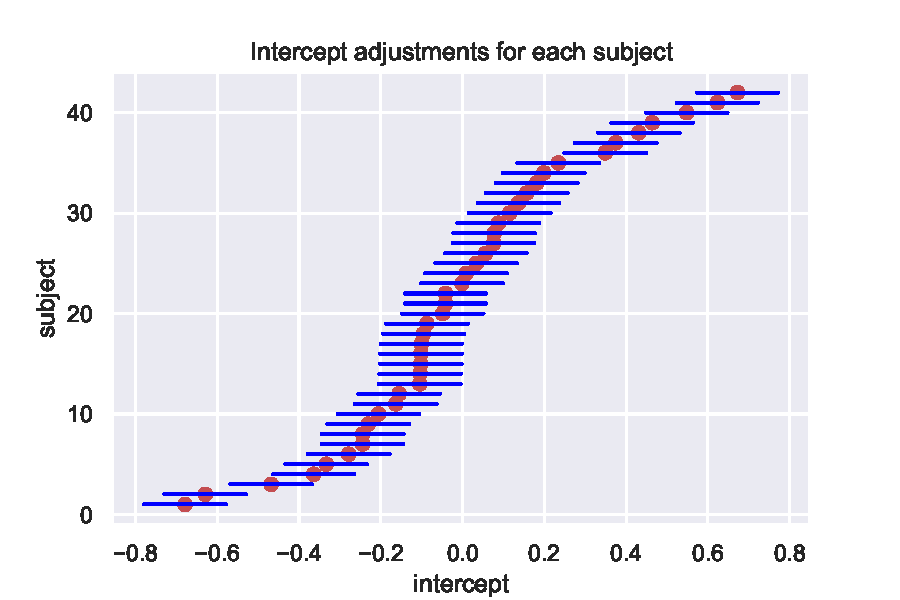
\includegraphics[scale=.65]{./images/model1_inter.pdf}
    \caption{Representation of the intercept adjustements by subject.}
    \label{fig:model1}
\end{figure}

In the Figure \ref{fig:model1}, we can note that our model produces a different intercept for each subjects in addition to a parameter estimate for features logrt (log-transformed reading time) and so (the contrast coding) which is constant between subjects. In addition, the error bars represent $95\%$ confidence intervals. We can see that there is a large variability in the average reading times between subjects.

 \subsection{Criterion AIC}
In order to evaluate the models, we will use the AIC criterion.
We will calculate the AIC of the model above to compare it with those of the other models defined in the other parts below. The AIC criterion is defined by:
\[ AIC = 2k - 2\ln({\hat{L}}),\]
with  $k$ is the number of estimated parameters in the model and $\hat{L}$ is the maximum value of the likelihood function for the model.


For practical reasons, we will use the AIC formula defined using the deviance.
We have the formulas below:
$$\text{deviance}= 2 \times \log(\text{likelihood}),$$ 
$$AIC=\text{deviance} + 2 \times (p+1),$$
with p is the number of parameters in the model. In the formula of AIC, $1$ is for the estimated residual variance and $p$ is all the other parameters.


Using the above formula and for our associated model, we find an AIC of approximately $719.6$ (with a total of $4$ parameters which corresponds to $3+1$).

\subsection{Model validation}
We will now see how can we validate the model. In order to check the homogeneity, we plot the predicted values versus the residuals.
\begin{figure}[H]
    \centering
    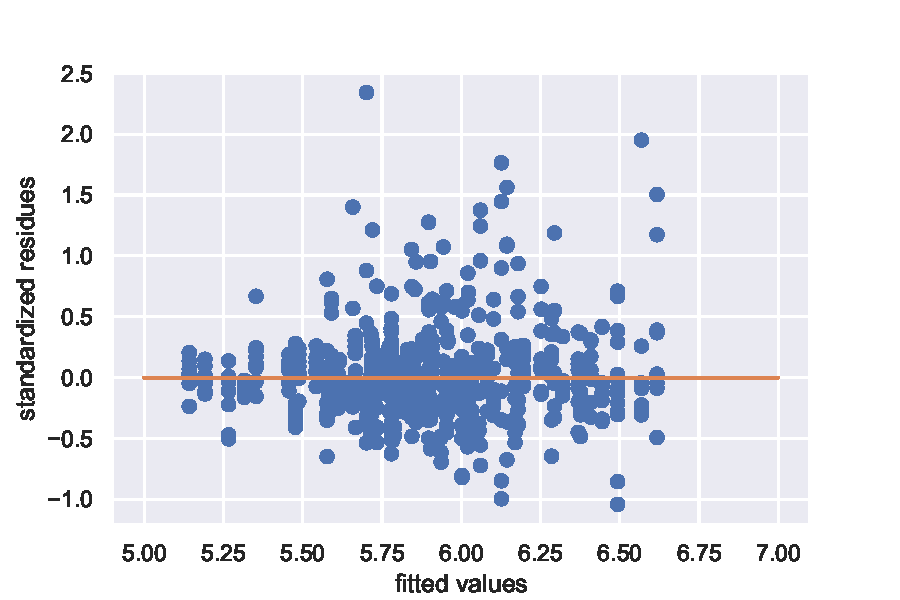
\includegraphics[scale=.65]{./images/homo_mod1.pdf}
    \caption{Representation of the predicted values as a function of 
residual values.}
    \label{fig:homo_mod1}
\end{figure}

In the Figure \ref{fig:homo_mod1}, we can note that the magnitude of the residuals suggests that the model seems to model our data well.

We can also check the normality of the residuals.
\begin{figure}[H]
    \centering
    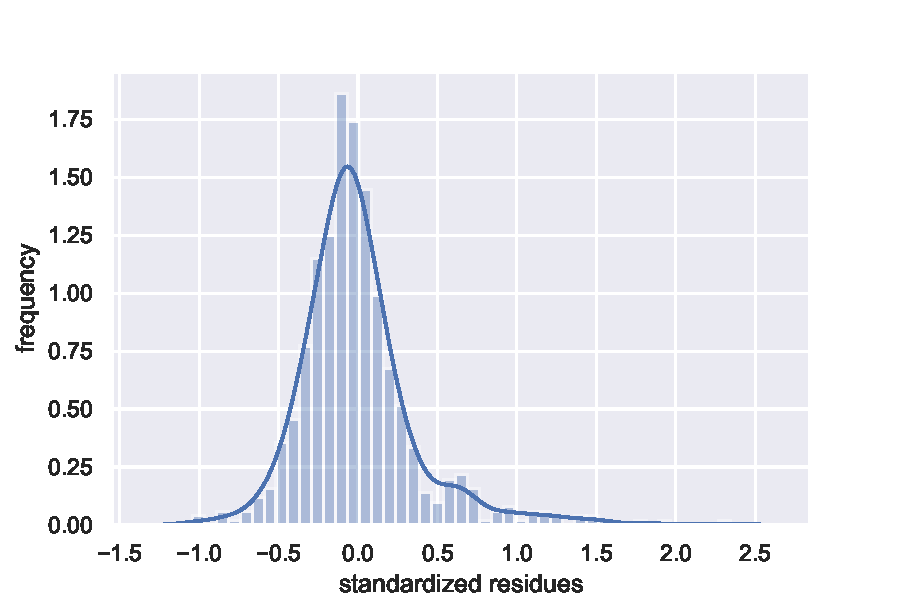
\includegraphics[scale=.65]{./images/resid_norm.pdf}
    \caption{Representation of the normality of the residuals.}
    \label{fig:resid}
\end{figure}

%%%%%%%%%%%%%%%%%%%%%%%%%%%%%%%%%%%%%%%%%%%%%%%%%%%%%%%%%%%%%%%%%%%%%%%%%%%%%%%
%%%%%%%%%%%%%%%%%%%%%%%%%%%%%%%%%%%%%%%%%%%%%%%%%%%%%%%%%%%%%%%%%%%%%%%%%%%%%%%

%%%%%%%%%%%%%%%%%%%%%%%%%%%%%%%%%%%%%%%%%%%%%%%%%%%%%%%%%%%%%%%%%%%%%%%%%%%%%%%
%%%%%%%%%%%%%%%%%%%%%%%%%%%%%%%%%%%%%%%%%%%%%%%%%%%%%%%%%%%%%%%%%%%%%%%%%%%%%%%
\section{Model type $2$: Varying intercepts and slopes, without a correlation}

The first model suppose different intercepts by subjects. However, the slope remained the same for each subject. So, we will now study a second type of model by varying the intercepts and slopes, without correlation. 
As with the intercepts, only the mean and standard deviation of the slopes are estimated instead of $42$ separate slopes.

\subsection{Mathematical equation of the model}
The mathematical equation of the model is:
\[y_{ij}= \beta_0 + u_{0i} + (\beta_1 + u_{1i}) \times so_{ij} + \varepsilon_{ij},\]
In this model, $i$ indexes subjects and $j$ indexes items.
The model has a different intercept $\beta_0 + u_{i0}$ for each subject $i$.

In the model above, we have three sources of variance which are :
\begin{itemize}
    \item $u_0 \sim \mathcal{N}(0,\sigma_{u0})$,
    \item $u_1 \sim \mathcal{N}(0,\sigma_{u1})$,
    \item $\varepsilon \sim \mathcal{N}(0, \sigma)$ the noise.
\end{itemize}

The output of the model is:
\begin{center}
    \begin{tabular}{|c|c|c|c|c|}
    \hline
         & Coef & Std.Err & z & P>|z|   \\
         \hline \hline
        Intercept & 5.883 & 0.051 & 115.496 & 0.000\\
         so & 0.062 & 0.022 & 2.810 & 0.005  \\
         Group var &  0.101 & 0.068 &  & \\
         Group x so Cov & 0.020 & 0.022 & & \\
         so Var & 0.012 & 0.013 & & \\
         \hline
    \end{tabular}
    \captionof{table}{Numerical outputs of the mixed linear model carried out on \texttt{Python}.} 
\end{center}

In order to determine if the slope is significantly different from $0$ or not, we will study its confidence interval.
Indeed, if its confidence interval includes the value $0$, we can say that at the $5\%$ threshold, the slope is not significantly different from $0$.
The confidence interval of the slope is $[0.062-0.022 \times 1.96, 0.062+0.022 \times 1.96]=[0.019, 0.105]$. So, as the latter does not include $0$, we can affirm at the $5\%$ threshold that the slope is significantly different from $0$.

Let's visualize the adjustments to the intercept and slope for each subject.

\begin{figure}[H]
    \centering
    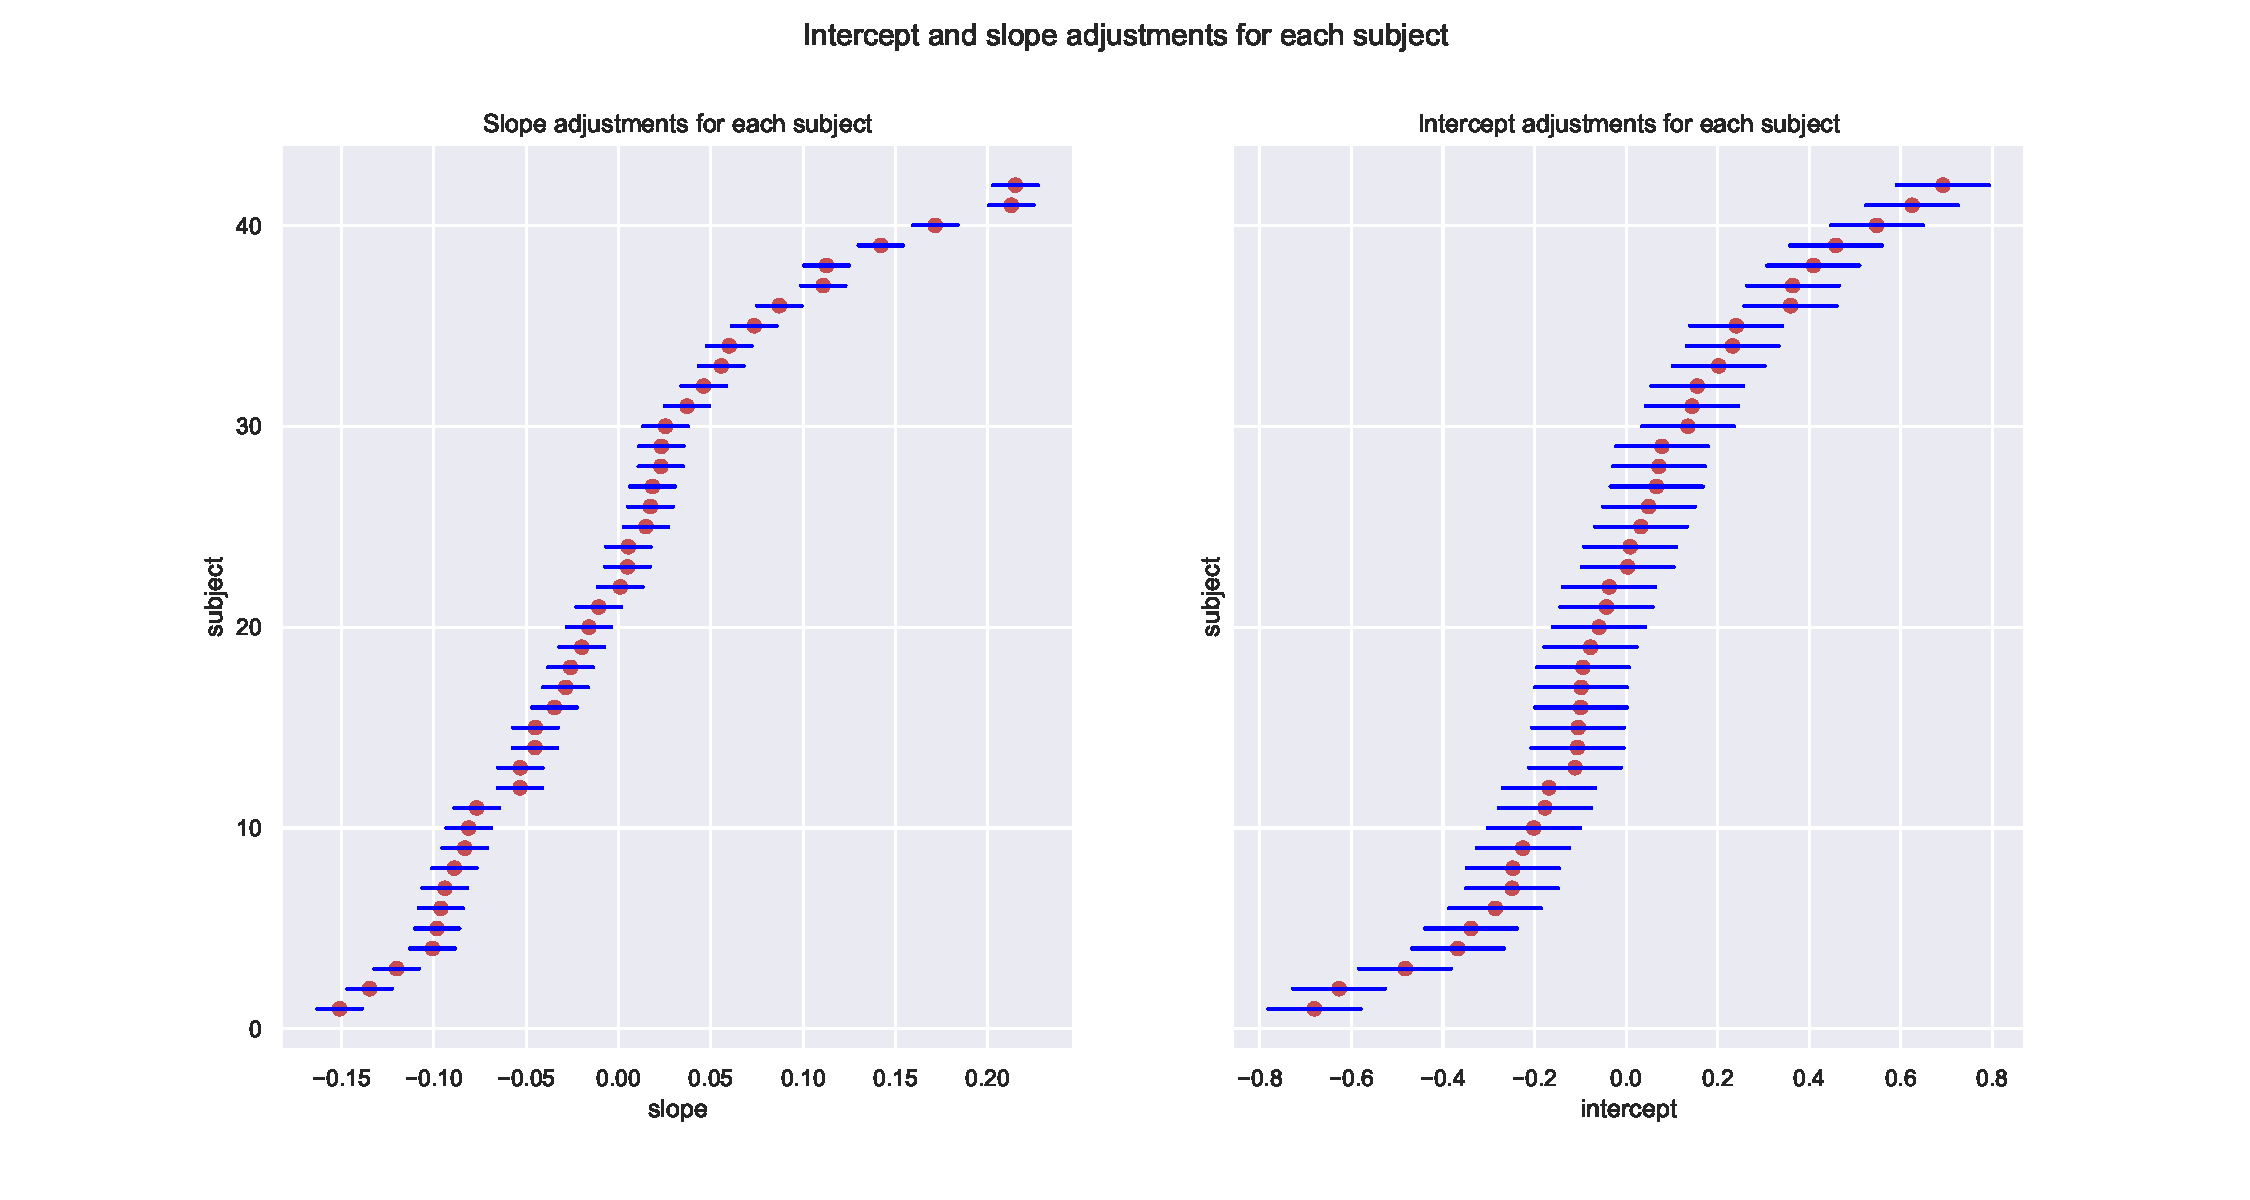
\includegraphics[scale=.42]{./images/model2_inter.pdf}
    \caption{Representation of the intercept and slope adjustements by subject.}
    \label{fig:model2}
\end{figure}

In the Figure \ref{fig:model2}, we can note a little variation in slope between subjects. However, there is a large variability in the average reading times between subjects. Like the previous model, we can note that our model produces a different intercept and slope for each subjects in addition to a parameter estimate for features logrt (log-transformed reading time) and so (the contrast coding) which is constant between subjects. The error bars in the figure represent $95\%$ confidence intervals.

\subsection{Criterion AIC}
After studying two different models, we can compare these two models by comparing their AIC values.
Using the AIC formula defined from the deviance, we obtain an AIC of approximately $711.146$. 
Since the previous model has a greater AIC value than this, we can say that this model is the "best" model for our data. Thus, this model has a greater predictive power than the previous model.

\subsection{Model validation}
As before, we will try to validate our model.
We are going to plot the predicted values versus the residuals to check the homogeneity.
\begin{figure}[H]
    \centering
    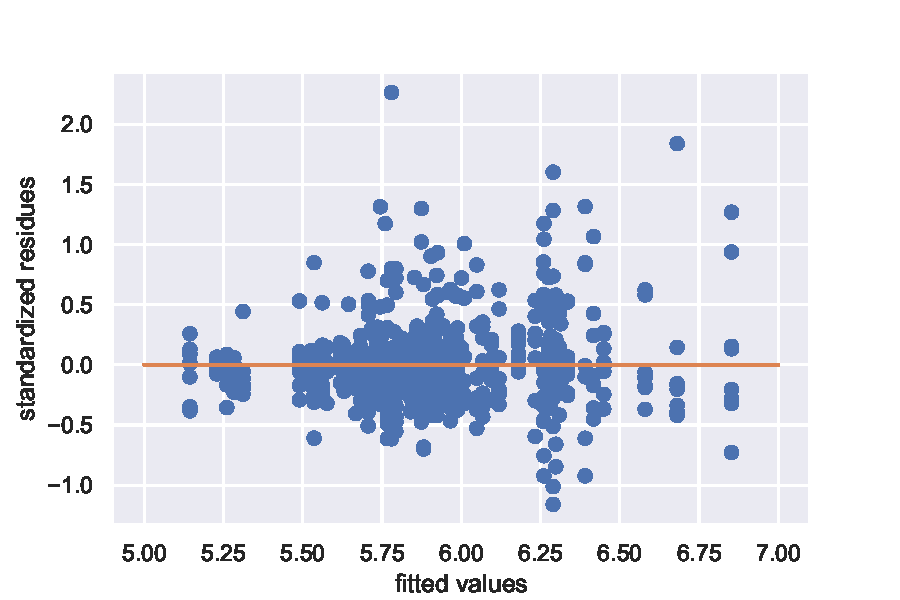
\includegraphics[scale=.65]{./images/homo_mod2.pdf}
    \caption{Representation of the predicted values as a function of 
residual values.}
    \label{fig:homo_mod2}
\end{figure}

In the Figure \ref{fig:homo_mod2}, we can note that the magnitude of the residuals suggests that the model seems to model our data well.

Let us come to the normality of the residues
\begin{figure}[H]
    \centering
    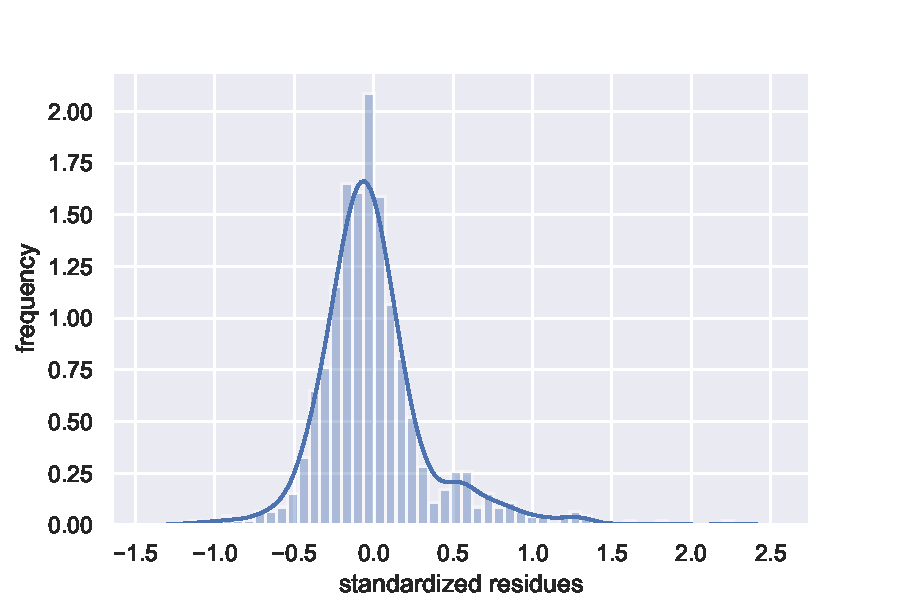
\includegraphics[scale=.65]{./images/resid_norm_m2.pdf}
    \caption{Representation of the normality of the residuals.}
    \label{fig:residm2}
\end{figure}


%%%%%%%%%%%%%%%%%%%%%%%%%%%%%%%%%%%%%%%%%%%%%%%%%%%%%%%%%%%%%%%%%%%%%%%%%%%%%%%
%%%%%%%%%%%%%%%%%%%%%%%%%%%%%%%%%%%%%%%%%%%%%%%%%%%%%%%%%%%%%%%%%%%%%%%%%%%%%%%


%%%%%%%%%%%%%%%%%%%%%%%%%%%%%%%%%%%%%%%%%%%%%%%%%%%%%%%%%%%%%%%%%%%%%%%%%%%%%%%
%%%%%%%%%%%%%%%%%%%%%%%%%%%%%%%%%%%%%%%%%%%%%%%%%%%%%%%%%%%%%%%%%%%%%%%%%%%%%%%
\section{Model type 3: Varying intercepts and varying slopes, with correlation}
%%%%%%%%%%%%%%%%%%%%%%%%%%%%%%%%%%%%%%%%%%%%%%%%%%%%%%%%%%%%%%%%%%%%%%%%%%%%%%%
%%%%%%%%%%%%%%%%%%%%%%%%%%%%%%%%%%%%%%%%%%%%%%%%%%%%%%%%%%%%%%%%%%%%%%%%%%%%%%%

%%%%%%%%%%%%%%%%%%%%%%%%%%%%%%%%%%%%%%%%%%%%%%%%%%%%%%%%%%%%%%%%%%%%%%%%%%%%%%%
%%%%%%%%%%%%%%%%%%%%%%%%%%%%%%%%%%%%%%%%%%%%%%%%%%%%%%%%%%%%%%%%%%%%%%%%%%%%%%%
\section{Conclusion}
%%%%%%%%%%%%%%%%%%%%%%%%%%%%%%%%%%%%%%%%%%%%%%%%%%%%%%%%%%%%%%%%%%%%%%%%%%%%%%%
%%%%%%%%%%%%%%%%%%%%%%%%%%%%%%%%%%%%%%%%%%%%%%%%%%%%%%%%%%%%%%%%%%%%%%%%%%%%%%%

%%%%%%%%%%%%%%%%%%%%%%%%%%%%%%%%%%%%%%%%%%%%%%%%%%%%%%%%%%%%%%%%%%%%%%%%%%%%%%%
%%%%%%%%%%%%%%%%%%%%%%%%%%%%%%%%%%%%%%%%%%%%%%%%%%%%%%%%%%%%%%%%%%%%%%%%%%%%%%%
\section{Bibliography}
\nocite{*}
\printbibliography
%%%%%%%%%%%%%%%%%%%%%%%%%%%%%%%%%%%%%%%%%%%%%%%%%%%%%%%%%%%%%%%%%%%%%%%%%%%%%%%
%%%%%%%%%%%%%%%%%%%%%%%%%%%%%%%%%%%%%%%%%%%%%%%%%%%%%%%%%%%%%%%%%%%%%%%%%%%%%%%

\end{document}